%
% Compile with
%
%   latexmk -pdf --shell-escape brennstab.tex
%
\documentclass[crop,tikz,border=10pt, convert={density=150,size=1080x800,outext=.png}]{standalone}

\usepackage{tikz}
\usetikzlibrary{arrows,
		calc,
		decorations.pathmorphing,
		decorations.markings,
		patterns}
\usepackage[utf8]{inputenc}
\usepackage[T1]{fontenc}

\begin{document}
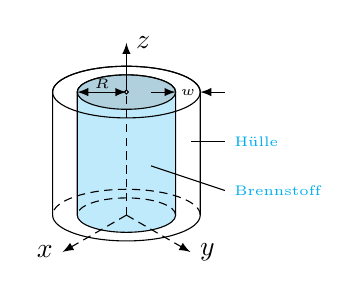
\begin{tikzpicture}[scale=1.25]

\draw [fill=cyan, fill opacity=.25]
  (180:5mm) coordinate (a)
  -- ++(0,-12.5mm) coordinate (b)
  arc (180:360:5mm and 1.75mm) coordinate (d)
  -- (a -| d) coordinate (c) arc (0:180:5mm and 1.75mm);
  \draw [fill=gray, fill opacity=.25]
  (0,0) coordinate (t) circle (5mm and 1.75mm);
  \draw [densely dashed] (d) arc (0:180:5mm and 1.75mm);
  \draw []
  (180:7.5mm) coordinate (A)
  -- ++(0,-12.5mm) coordinate (B)
  arc (180:360:7.5mm and 2.625mm) coordinate (D)
  -- (A -| D) coordinate (C) arc (0:180:7.5mm and 2.625mm);
  \draw []
  (0,0) coordinate (T) circle (7.5mm and 2.625mm);
  \draw [densely dashed] (D) arc (0:180:7.5mm and 2.625mm);
  \draw [densely dashed ]
  ([yshift=-12.5mm]T) coordinate (B)
  edge [-latex] node [pos=1, right] {$y$} +(-30:7.5mm)
  edge [-latex] node [pos=1, left] {$x$} +(-150:7.5mm)
  -- (T)  node [anchor=center, circle, draw, solid, inner sep=.5pt, fill=white] {} edge [solid, -latex] node [right, pos=1] {$z$} ++(0,5mm) ;
  
\draw (0.25,-0.75) -- (1,-1) node[right] {\tiny \textcolor{cyan}{Brennstoff}};
\draw (0.66,-0.5) -- (1,-0.5) node[right] {\tiny \textcolor{cyan}{H\"ulle}};

\draw[latex-latex] (0,0) -- (-0.5, 0) node[midway, above, inner sep=1pt] {\tiny $R$};

\draw[-latex] (0.25, 0) -- (0.5, 0);
\draw[latex-] (0.75, 0) -- (1, 0);
\node at (0.625, 0) {\tiny $w$};

\end{tikzpicture}
\end{document}